\documentclass{article}
\usepackage[margin=1in]{geometry}
\usepackage[utf8]{inputenc}
\usepackage{qtree}
\usepackage{setspace}
\usepackage{amsfonts}
\usepackage{mathtools}
\usepackage{amsmath}
\pagenumbering{arabic}
%\doublespacing
\setlength{\parskip}{5pt}
\usepackage{fancyhdr}
\newcommand{\sample}{\xleftarrow{\$}}
\usepackage{graphicx}
\usepackage{lastpage}
\newtheorem{theorem}{Theorem}
\title{Morse Theory and Linkages}
\author{Vickram Rajendran}
\date{December 2017}

\begin{document}

\maketitle
\pagestyle{fancy}
\fancyhf{}
\rhead{Topics in Geometry}
\lhead{Morse Theory and Linkages}
\rfoot{Page \thepage \hspace{1pt} of \pageref{LastPage}}
\section{Introduction}
A linkage is a system of "bars", connected to each other only at their endpoints, such that each bar has a specified length.  Since the early 1500's, linkages have been used to model physical and mechanical phenomena. For instance, linkages have been used to model things like steam engines, joysticks, walking machines, and to convert circular motion to straight-line motion. 

To formalize the idea of a linkage, we define a linkage with bar lengths $l_1, l_2, \cdots, l_n$, with each $l_i > 0$, as $\mathcal{L} = (l_1, l_2, \cdots, l_n)$. Then the space of possible configurations of a planar linkage $\mathcal{P(L)}$ is a set of points in $\mathbb{R}^{2n} = (p_1, p_2, \cdots, p_n)$ where $|p_i - p_{i-1}| = l_i$. Given a linkage, a natural question is what the space of possible configurations of the linkage looks like - this has applications in engineering to determine the degrees of freedom of a system, or to determine whether certain configurations are reachable from other configurations. A quick application of the Regular Value Theorem shows that the configuration space is usually a manifold, the details of which can be found in \cite{spherical} or \cite{planar}. In particular, we are concerned with finding the topology of a configuration space of a linkage. We will focus on planar closed chains, where the bars form a planar polygon. This is formally defined as $p_n = p_1$, and $p_i \neq p_j$ for all other $1 \leq i, j \leq n$.  In this context, translations and rotations of the entire linkage yield the same configuration, so we will identify all translations and rotations of a particular configuration. This means we only need to consider linkages where the first bar lies on the positive x-axis and starts at the origin, or $p_0 = (0, 0), p_1 = (l_1, 0)$. 

In this paper, we use Morse Theory to analyze the topology of a configuration space of linkages. First, a brief introduction to Morse Theory is given. We then show a natural Morse function that has the configuration space as a level set, and explain the standard method to find the topology of a configuration space for planar polygons, though a similar method extends for other linkages. We compare this to other methods used to find the same topology, such as the fibred product approach. Finally, we show generalizations of the Morse theoretic approach to computational origami and to cyclic polygons. 

\section{Morse Theory}
Morse Theory is an approach from differential topology that studies the topology of a space $M$ by looking at differentiable functions from that space. The idea is to look at the level sets of a function from $M \to \mathbb{R}$, and look at how the topology of the level sets change as we move along $\mathbb{R}$. Morse's crucial insight was that the topology of the level set should be exactly the same unless we pass specific points on $\mathbb{R}$, and more than that, we can predict how the topology changes through these points by classifying them.  
\begin{figure}[!ht]
    \centering
    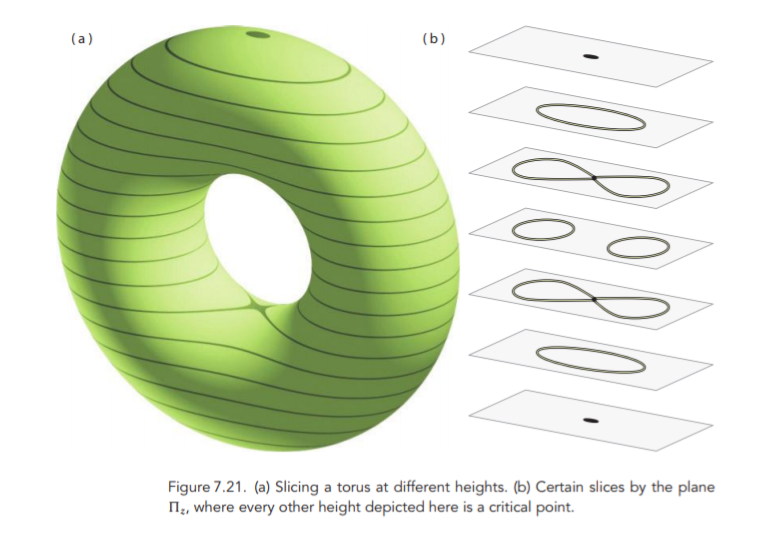
\includegraphics[scale = .4]{morse.png}
    \caption{A Morse Function that looks at level sets $f^{-1}(z) $\cite{rourke}}
    \label{fig:my_label}
\end{figure}
To formalize this, we begin with some definitions. If we have a smooth function $f: M \to \mathbb{R}$ on a differentiable manifold $M$, and $df$ the differential, then we let the points $x \in M$ where $df(x) = 0$ be \textbf{critical points}, and the points $f(x)$ are \textbf{critical values} of $f$. If the Hessian matrix at $x$ is nonsingular, then the point $x$ is said to be a \textbf{non-degenerate} critical point. A \textbf{Morse function} is a function that has only non-degenerate critical points. 

While studying these Morse functions have incredible and extensive applications, we require only a few theorems - proofs of these theorems and many of these applications are in \cite{milnor}. \\ \\
\textbf{Theorem 1.} \emph{Suppose f is a smooth real-valued function on $M$, the interval $[a, b]$ has no critical values, and $f^{-1}[a, b]$ is compact. Then $f^{-1}(-\infty, a]$ is homeomorphic to $f^{-1}(-\infty, b]$.}
\\ \\
A standard example of a Morse Function is the height function for surfaces, $f(x, y) = z$. This is the function that embeds a surface, which can always be parametrized with two variables, into $\mathbb{R}^3$ and outputs the height of each particular point in the surface. In Figure 1, we see this Morse function in action. The critical values of this function are the top of the torus, the top of the hole, the bottom of the hole, and the bottom of the torus. Then the theorem predicts that if $z = (a, b)$ is in between any two adjacent critical values, the level set for $f^{-1}(z)$ is topologically the same for all $z \in (a, b)$. We can easily verify this. The level-set for $z$ above the torus is just the empty set. In between the top of the torus and the top of the hole, the level set is consistently topologically equivalent to a circle. This same trend continues, as the topology between the top of the hole and the bottom of the hole is two disconnected circles, and so on. 
\\ \\
At this point, we might notice that while the topology is not the same between critical points, it might change in some predictable ways. In particular, we define the \textbf{index} of a critical point to be the dimension of the largest negative-definite submatrix in the Hessian at that critical point. Intuitively, this describes the amount of dimensions that the morse function is decreasing in at this critical point. As an example, we can use this heuristic to compute the index at each of the four critical points in the torus example. At the top of the torus, the height is decreasing in all directions, so there are two dimensions that it is decreasing in - thus it has index $2$. At the top of the hole, the height is decreasing along a circle around the hole, but the height is increasing along a circle around the body of the torus - so it has index $1$. Similarly, at the bottom of the hole the same thing is happening, but the height is increasing along the hole and decreasing along a circle around the body of the torus. Finally, the bottom of the torus has index $0$ since the height is non-decreasing in all directions from here. 
\\ \\
Naturally, we hope that we can predict changes in the topology through a critical point just by looking at the index of a critical point. Indeed, that turns out to be the case. \\ \\
\textbf{Theorem 2.} \emph{Suppose $f: M \to \mathbb{R}$ is smooth, and $x$ is a non-degenerate critical point of $f$ with index $n$. Let $f(x) = y$. Let $\epsilon > 0$ such that $f^{-1}[y - \epsilon, y + \epsilon]$ is compact and has no other critical points except for $x$. Then $f^{-1}(-\infty, y + \epsilon]$ is homotopy equivalent to $f^{-1}(-\infty, y - \epsilon]$ with an $n$-cell attached.}
Again, the details of this theorem are in \cite{milnor}. 

These theorems are all we will need to use Morse Theory.

\section{Morse Theory on Configuration Spaces}
We return to the area of linkages. Recall that the configuration space of a planar linkage $\mathcal{L} = (l_1, l_2, \cdots , l_n)$ is defined as a set $\mathcal{P(L)}$ of points $p \in \mathbb{R}^{2n}$ where $p = (p_1, p_2, \cdots, p_n) \in \mathcal{P(L)}$, with each $p_i = (x_i, y_i)$, if $|p_i - p_{i-1}| = l_i$ for all $i$. Since configurations of linkages are the same up to translation, we mandate that $p_1 = 0$ to identify all of these. In order to use Morse Theory, we want to find a Morse function $f$ from some space $M \to \mathbb{R}$ such that a level set of this Morse function turns out to be exactly the configuration space of the linkage.

The standard approach, done essentially the same way in \cite{planar}, is to allow one of the bar lengths to vary. Then we consider the space $M = \bigcup_{z>0} \mathcal{P(L)}_z$, where $\mathcal{P(L)}_z$ is the configuration space of the linkage $\mathcal{L}_z = (l_1, l_2, l_3, \cdots, z)$. The Morse function we will use is just $f: M \to \mathbb{R}$, defined as $f(x) = z$, where $z = |p_2|$, where the $p_i$ are the points in the configuration $x$. $z$ is the length of the first bar, and so the level set $f^{-1}(l_1)$ should be the configuration space of a linkage with first bar having length $l_1$, which is exactly what we are looking for. A point worth noting is that the choice of which bar length to vary should not matter, the choice of $l_1$ was arbitrary, though the analysis of indices become slightly different.

We will examine this formulation for a closed chain. In this case, we also necessitate that the first bar lies along the $x$-axis starting at the origin since the configurations of the linkage is invariant up to rotation and translation. The same Morse function applies. We define a \textbf{straight line configuration} to be a configuration $x \in M$ where each $p_i$ of $x$ lies on the $x$-axis. We have two theorems here, both proven in \cite{planar}, that summarize the findings for closed chains.
\\ \\
\textbf{Theorem 3.} \emph{The critical points of $f$ are precisely the straight line configurations.}
\\ \\
\textbf{Theorem 4.} \emph{Let $l$ be the number of edges that go to the left in a straight line configuration $c$. Then the index of $c$ is $l - 1$.}
These are essentially propositions $2, 5$ in \cite{planar}, and the proofs are a straight-forward calculations of the Hessian and the derivative with local coordinates, the details of which are in \cite{planar}. 

The idea, at this point, is to begin looking at the level set at a point $z$ large enough such that $f^{-1}(z) = \emptyset$. Then as we bring $z$ closer to $l_1$, we track the changes in the topology of the configuration space, at each critical point we hit. Once we reach $z = l_1$, we will then have an idea of what the topology of the configuration space is.

Let us apply this to an example of the equilateral pentagon, the linkage $\mathcal{L} = (1, 1, 1, 1, 1)$, with the morse function $f$ described above on $M$. Then note that any straight line configuration must have an integer coordinate for the first bar, since other wise the sum of the lengths would not get back to the origin. Also, the length of the first bar must be an even integer, since otherwise we would not be able to use the four remaining bars, all of the same length, to go back to the origin. Finally, note that if $z > 4$, then the configuration space is empty since we can not use the remaining $4$ bars to come back to the origin. Thus the only possible critical values are $z = 4, 2, 0$. If $z = 4$, there is only one configuration since all of the remaining bars must point to the left. Also, the index of this critical point is $3$. If $z = 2$, then we have $4$ separate configurations, since any one of the remaining $4$ bars can point to the right, with the other three pointing to the left, so the index of each of these critical points is $2$.
\begin{figure}[!ht]
    \centering
    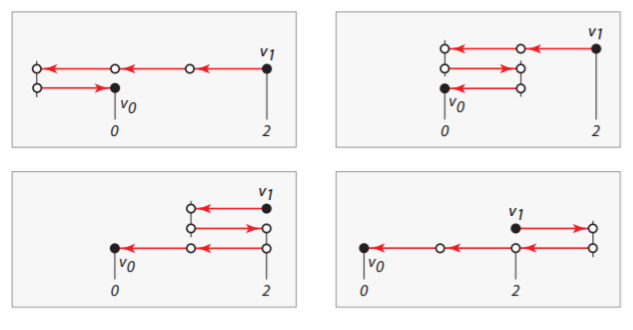
\includegraphics[scale = .5]{z2.png}
    \caption{The straight line configurations of the equilateral pentagon at $z = 2$ \cite{rourke}}
    \label{fig:z2}
\end{figure} 
If $z = 0$, then this means that $l_1 = 0$, which we said was not possible since we cannot have $l_i \leq 0$. So there are no configurations here. 

Thus as we start $z = z_0 > 4$, the configuration space is empty, and remains empty until we hit $z = 4$. This is an index $3$ critical point, so the homotopy type of the configuration space will be the same as three space without a $3-cell$, or a $3-$ dimensional ball, i.e., a sphere. Then the topology stays the same as a sphere until we get to the next critical value, which is $4$ critical points each of index $2$ at $z = 2$. For this, the difference between the homotopy type of the topologies is $4$ $2$ cells, since we have $f^{-1}(2 - \epsilon)$ with $4$ two cells is a sphere. We can model this by attaching handles, since adding a two cell would then just remove this handle. So we can say that $f^{-1}(2 - \epsilon)$ is a sphere with $4$ handles attached to it, which is just a surface of genus $4$, or by the classification of surfaces, a connected sum of $4$ tori. There are no more critical values on the way to $z = l_1 = 1$, so this is the topology of the configuration space of an equilateral pentagon, which can be verified is the correct topology in \cite{planar}. 

\section{Other Methods}
Another method to find the topology of the configuration space is the so-called fibred product approach, where one "cuts" the linkage and considers the possible configurations of the point that was cut on each side of the linkage. Then the intersection of those workspaces are the workspaces of the point, and counting how many configurations that the linkage has for each point in that workspace can give an idea of the topology of the configuration space. 
\begin{figure}[!ht]
    \centering
    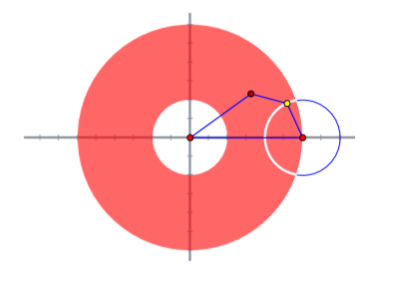
\includegraphics[scale=.5]{fibred.jpg}
    \caption{The fibred product approach for a quadrilateral. (picture from slides)}
    \label{fig:fibred}
\end{figure}\cite{spherical}
Note that disconnecting the linkage at the yellow point $p_3$ means that $p_3$ can effectively be considered as the end point of two separate open chains, one with two bars starting from the origin $(l_3, l_4)$, and one with one bar starting from the right endpoint of the bar along the origin. In the first case, the yellow point must lie in the annulus of radii $r_1 = |l_4 - l_3|, r_2 = |l_4 + l_3|$, where the numbering convention is the same as above. This is depicted in red in the figure. In the other case, we see that since $p_1$ is pinned at $(l_1, 0)$, there is only one bar that is constraining $p_3$, and so it must lie in a circle of radius $r = l_2$. Since both cases must be true at the same time, the intersection of the annulus and the circle are the only possible locations for $p_3$. 

We can use this to find the topology of the configuration space If $p_3$ is not on the boundary of the annulus, then there are two configurations of $l_3, l_4$ that lead to it - One where the bars make a left turn and one where they make a right turn. However, when $p_3$ is on the boundary, there is only one configuration since $l_3, l_4$ must be in a straight line. So the configuration space consists of the circular arc, but each point interior to the circular arc has two configurations since it is inside the annulus. Thus the configuration space is identifying two separate circular arcs at the endpoints individually (since there is only one configuration for each endpoint of the arc), creating a circle.

Unfortunately, this method breaks down with more complicated linkages - it becomes very difficult to count all of the possible ways that a configuration can occur, even if there is only one point being considered. Also, it requires splitting the linkage into more simplistic linkages, which might be difficult to do. More complex linkages also have nontrivial ways to cut and paste the various configurations together - this case was easy as we just identified two points on a circle, and the five-bar case also isn't too bad since we can use this as a polygonization and calculate the Euler characteristic, but the method is very difficult to follow afterwards. Morse theory provides an intuitive alternative that doesn't require as much of a brute force technique or cutting and pasting techniques in order to talk about the topology of the configuration space. 

\section{Further Work}
Morse Theory has been used in a plethora of different ways to analyze the topology of configuration spaces. One particularly interesting application involves spherical linkages. In this model, the bar lengths are specified as the length of geodesics on a sphere, and all points must lie on the sphere. We can construct Morse functions in the same way as we did for planar linkages, and use them to analyze the configuration spaces, as done in \cite{spherical}. As one might expect from our analysis here, the critical points of a spherical linkage turn out to be the configurations that lie on a great circle, and this would likely generalize to any configuration that lies along a geodesic if we were dealing with linkages on a different Riemannian manifold. \cite{spherical} provides insight and intuition about the indices of the critical points in this context, and how the topology changes in each case. This example of spherical linkages is particularly interesting since rigid origami can be modelled by the use of spherical linkages. Thus Morse Theory is a powerful tool to study the configuration spaces of rigid origami. 

Another extension to Morse theory on linkages is to consider a different Morse function - our goal in this paper was to understand the configuration space of a linkage, but perhaps we wanted to study the space of linkages that all have a certain area or volume. We can construct a Morse function that defines the signed area of a planar linkage, and then apply Morse theory onto this function to uncover information about this space. This is explored much further in \cite{zhukova}, where it is shown that the critical points of this function are precisely the cyclic polygonal configurations. Zhukova also provides a simple formula for calculating the index of each critical point, allowing for a similar analysis to the one we did in this paper in order to discover information about the topology of this space.  
\section{Conclusion}
Morse Theory is a powerful and versatile tool to study the topology of linkages' configuration spaces. It provides an easy, algorithmic method of determining the topology without having to worry so much about counting the amount of configurations that every possible event can occur. By reducing the problem of topology to that of differential calculus and critical points, we can isolate specific areas where the topology will change and classify them accordingly. The ideas extend far beyond planar linkages, and can even be applied to seemingly unrelated concepts like origami. Morse theory provides a more nuanced and comprehensive discussion about linkages, and allows for greater insight into the underlying differential topology of the configurations of linkages. 


\bibliographystyle{abbrv}
\bibliography{bib}
\end{document}

